% !Mode:: "TeX:UTF-8"

\chapter{线程调度模块设计与实现}[thread]
\label{chapter:thread}

\section{模块概述}

进程是一个处于运行状态的程序实例,拥有自己的内存空间和运行时数据。Moonix采用了一个最简单的进程模型:进程和线程一一对应,即一个进程中只包含一个线程。这样,CPU实际上只是在调度线程,进程剥离出线程之后,就只剩下资源分配的属性了。Moonix中,一个进程保有一个页表和一个文件描述符数组:页表代表这个进程的独立的虚拟地址空间,文件描述符则表示这个进程打开的文件。

当一个线程运行时,CPU中的寄存器的值以及线程栈上的数据,称为这个线程的上下文。和中断类似,在线程切换时,需要将上一个线程的上下文保存起来,以便在未来再次切换到这个线程时,能够继续之前的状态运行下去。内核中线程的数据结构中保存了该线程的上下文地址,由于上下文总是存放在线程栈顶,所以该地址也是栈顶地址。

线程调度依赖于时钟中断。当时钟中断发生时,内核采用round robin算法,检查当前线程的时间片,并决定是否将暂停当前线程的运行,而将CPU资源让出。

Moonix中线程状态由线程池维护,线程的状态分为四种,分别如下:

\begin{itemize}
	\item 就绪状态(Ready):线程处于就绪队列中,等待被 CPU 调度执行
	\item 运行状态(Running):线程此时正占有 CPU 运行
	\item 睡眠状态(Sleeping):线程等待某个条件满足,此时线程不会被调度执行,直到条件满足后才会被加入就绪队列
	\item 退出状态(Exited):线程已经完成了任务执行,但是还没有回收资源
\end{itemize}

状态之间的切换及条件如图 \ref{pic:threadstatus} 所示。

\begin{figure}[htpb]
	\centering
	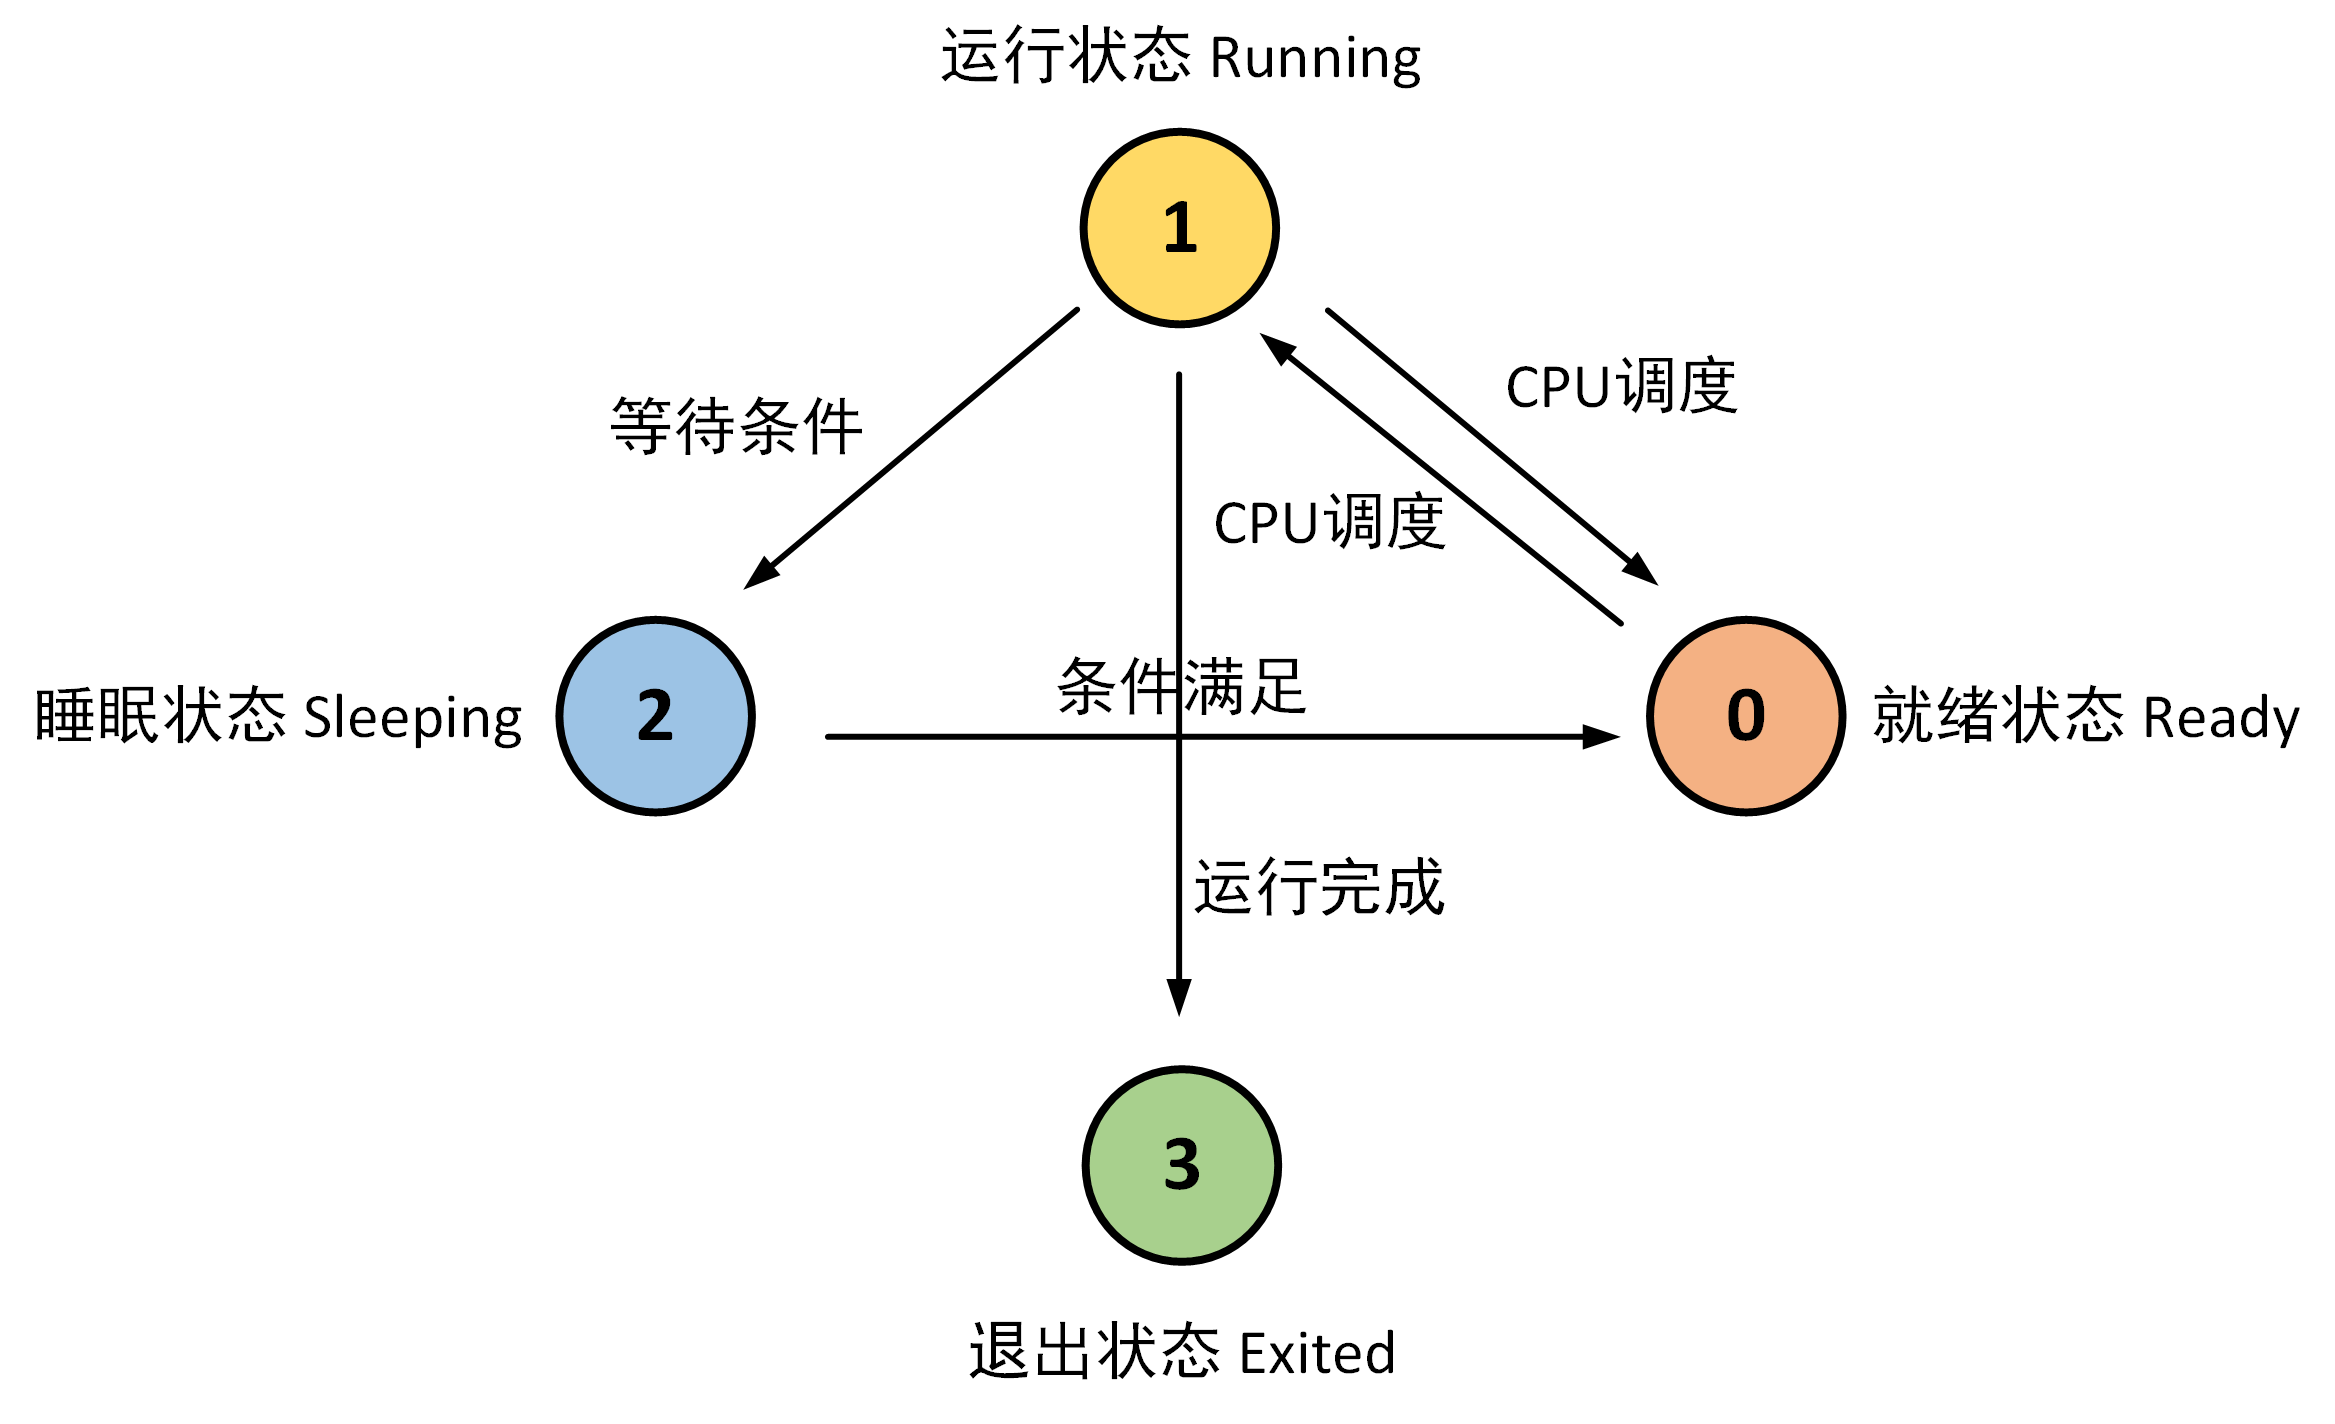
\includegraphics[width=0.45\textwidth]{threadstatus}
	\setlength{\abovecaptionskip}{2pt}
	\caption{保存中断上下文}
	\label{pic:threadstatus}
\end{figure}

\section{线程的启动和切换}

Moonix中将线程结构定义为如代码 \ref{lst:threadstructure} 的结构体。而实际上,在执行中,并不会用到kstack域,启动和切换基本只涉及contextAddr域。

\begin{figure}
\begin{lstlisting}[language={C}, caption={线程结构定义}, label={lst:threadstructure}]
typedef struct {
	usize contextAddr;  /* 线程上下文存储的地址 */
	usize kstack;       /* 线程栈底地址 */
} Thread;
\end{lstlisting}
\end{figure}

Moonix采用函数调用的方式进行线程上下文的切换,所以不需要像中断一样保存全部的通用寄存器。根据函数调用规范,在流程进入线程切换的函数时,就会自动保存调用者保存的寄存器到栈上。而在后续在切换回到该线程后,会首先从函数中返回,这部分寄存器的值会从栈上被恢复。所以,Moonix只需要手动保存以下的内容:

\begin{itemize}
	\item ra 寄存器,用于保存返回地址
	\item satp 寄存器,保存页表信息,本章的线程都可以说是同属于内核进程的,共用一个页表
	\item s0 ~ s11,函数调用中被调用者保存的寄存器
\end{itemize}

\begin{lstlisting}[language={C}, caption={线程上下文定义}, label={lst:threadcontext}]
typedef struct {
	usize ra;
	usize satp;
	usize s[12];
	InterruptContext ic;
} ThreadContext;
\end{lstlisting}

于是定义线程上下文如代码 \ref{lst:threadcontext}。除去上面说的三部分内容以外,还包含了一个中断上下文,严格来说这不属于线程运行上下文的一部分,Moonix会借助中断返回机制来初始化线程,这部分仅会在线程初始化时被保存在栈上,后续并不会被保存。

Moonix在启动后,实际上是位于一个启动线程中的。Moonix需要构造一个“静止”的线程,一个静止线程的结构看起来就像是刚刚被CPU抢断后保存的结构。这样,当其他正在运行的线程切换到它时,就可以将寄存器和栈变成预期的初始化状态,并且跳转到程序的入口开始运行。

Moonix在创建新线程时,会统一将线程的入口设置为\_\_interrupt函数,并填充InterruptContext中的寄存器的值。而线程的真正入口,则保存在InterruptContext中的sepc域中。

Moonix中断恢复的代码 \ref{lst:restorecontext} 逻辑中,中断恢复时会自动将栈顶的InterruptContext中的内容都恢复到寄存器中,并执行sret跳转到sepc寄存器中保存的地址处。而在进入新线程之前,内核就已经把ThreadContext压入到新线程的栈底,InterruptContext恰好位于栈顶。接下来的事情就顺理成章了:中断恢复函数会将InterruptContext中的内容全部恢复到CPU中,包括传入的参数和sepc,随后sret指令将流程跳转到sepc寄存器保存的地址处,即最初设置的线程的真正的入口处。sret指令还可以修改CPU的运行模式,可以通过修改sstatus寄存器的SPP位,来实现不同的运行模式下的线程。

\section{线程调度}

Moonix线程调度依赖于时钟中断,时钟中断的中断处理函数除去预约下一次时钟中断外,还会额外去进行线程调度的工作。

Moonix所有的运行流程都是运行在线程中的,由于要对所有的线程进行调度,Moonix创建了一个调度线程,专用于线程的切换与调度。Moonix中,这个线程被命名为Idle线程。具体来说,Idle线程的作用是:

\begin{enumerate}
	\item 当没有线程在运行时,调度线程根据一定的策略来选择一个线程来执行
	\item 当一个线程被调度器判断需要让出 CPU 控制权时,例如运行时间过长或者运行结束,并不是直接切换到另一个线程,而是先切换到这个调度线程,让调度线程根据一定的策略来选择另一个线程执行
\end{enumerate}

Moonix中定义了一个结构体Processor,用来保存调度线程参与调度所需要的所有信息,如代码 \ref{lst:processor}。其中idle字段就是调度线程,current字段描述了当前正在运行线程的信息,occupied字段表示当前是否有线程(除了调度线程)正在运行。Idle线程所有的调度都是直接依赖Processor结构进行的。

\begin{lstlisting}[language={C}, caption={Processor结构体}, label={lst:processor}]
typedef struct {
	ThreadPool pool;
	Thread idle;
	RunningThread current;
	int occupied;
} Processor;
\end{lstlisting}

Idle线程的入口点即为idleMain函数,如代码 \ref{lst:idlemain} 所示。

\begin{lstlisting}[language={C}, caption={idleMain函数}, label={lst:idlemain}]
void
idleMain()
{
	// 进入 idle 时禁用异步中断
	disable_and_store();
	while(1) {
		RunningThread rt = acquireFromPool(&CPU.pool);
		if(rt.tid != -1) {
			// 有线程可以运行
			CPU.current = rt;
			CPU.occupied = 1;
			printf("\n>>>> will switch_to thread %d in idle_main!\n", CPU.current.tid);
			switchThread(&CPU.idle, &CPU.current.thread);
			
			// 切换回 idle 线程处
			printf("<<<< switch_back to idle in idle_main!\n");
			CPU.occupied = 0;
			retrieveToPool(&CPU.pool, CPU.current);
		} else {
			enable_and_wfi();
			disable_and_store();
		}
	}
}
\end{lstlisting}

idleMain函数首先关闭中断响应,以防止调度过程被中断打断,造成混乱。接着尝试从线程池中获取一个可执行的线程,切换到该线程开始执行。当某个时刻时间片用完后,内核会切换回idle线程,流程会返回idleMain的第16行,并进入下一次循环。如果没有线程可供执行,idle线程会打开中断。

从一个正在运行的线程的角度来说,整个流程时间线如图 \ref{pic:threadswitch} 所示。

\begin{figure}[htpb]
	\centering
	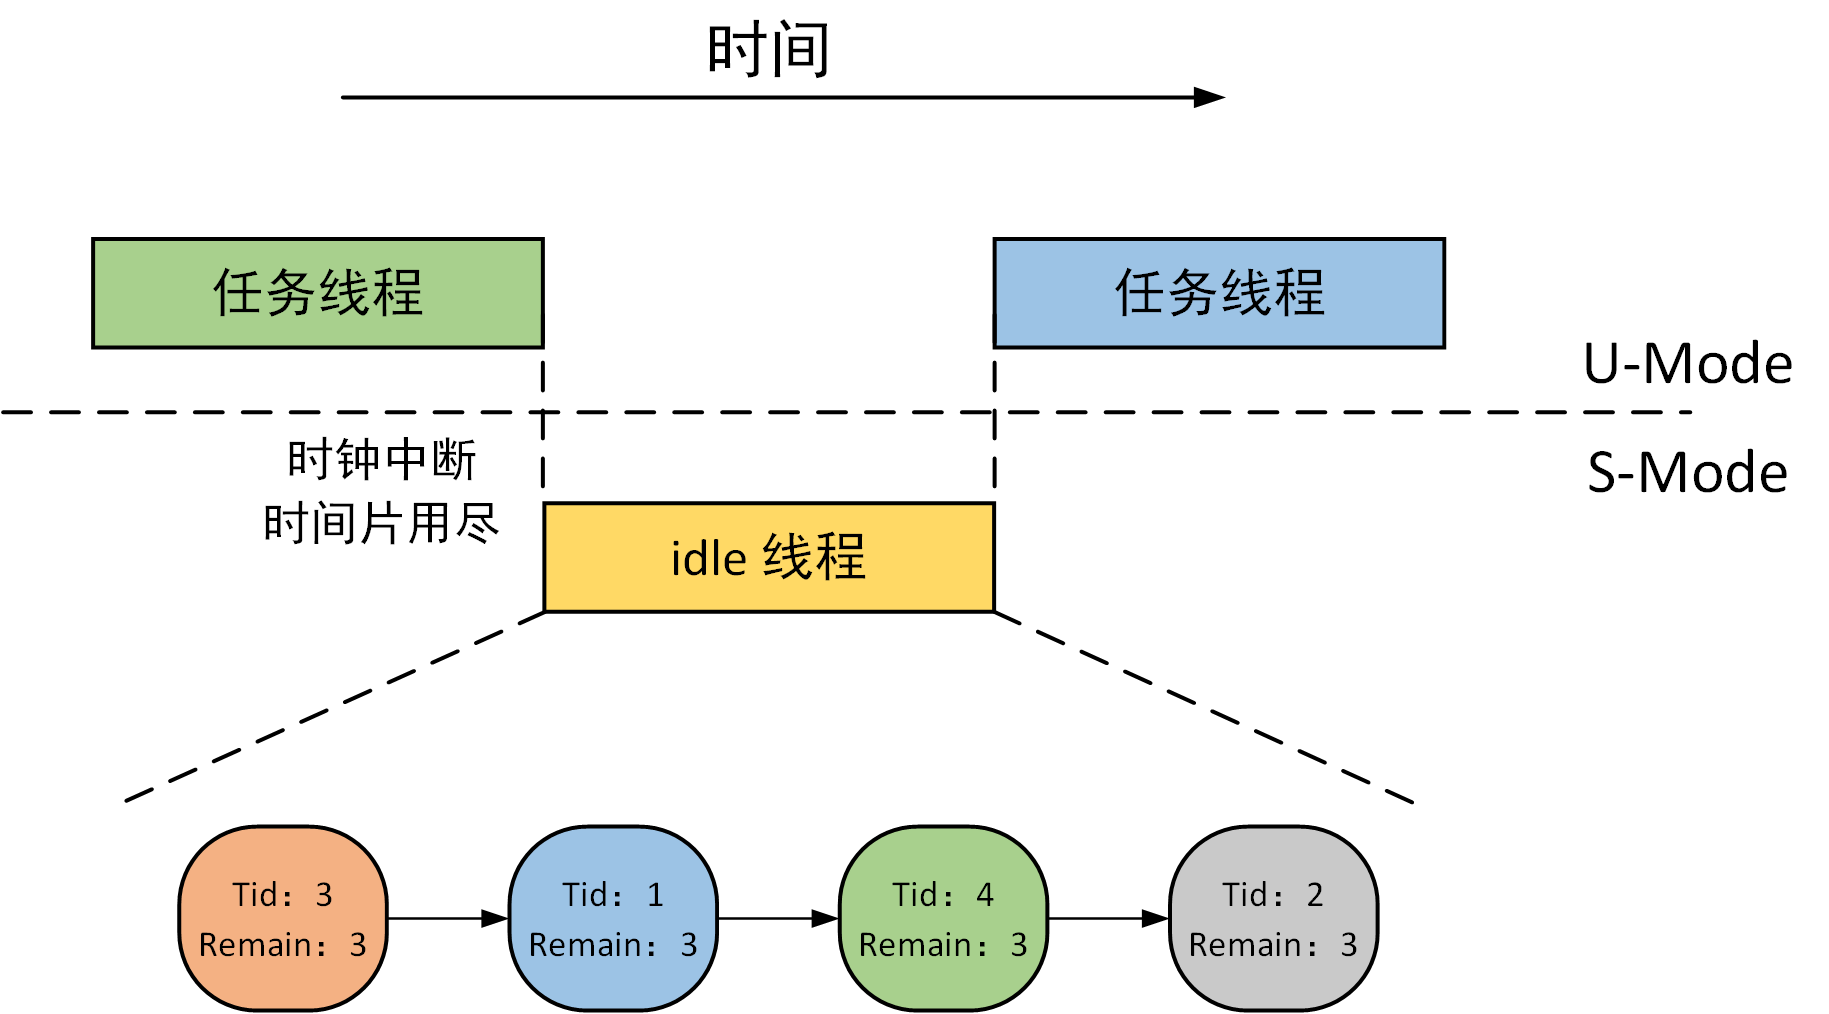
\includegraphics[width=0.6\textwidth]{threadswitch}
	\setlength{\abovecaptionskip}{2pt}
	\caption{线程切换时间线}
	\label{pic:threadswitch}
\end{figure}